\chapter{Detección óptica de caracteres (OCR)}
En este capitulo se pretende explicar que es el OCR, obtener una idea basica
de los distintos algorimos que se pueden implementar para
utilizar esta tecnica, para luego centrarnos en la red convolucional entrenada por
Ankandrew [referencia al git], con la idea de finalizar en un algoritmo en Python 3
que permita obtener los caracteres de una patente mediante una imagen.

\section{Algoritmos de OCR}
Como primera instancia vamos a definir que es OCR, por sus siglas en inglés Optical Character
Recognition o en español Reconocimiento Óptico de Carácteres, es una técnica que permite
obtener texto en formato ASCII a partir de una imagen.
Para logarlo se debe inspeccionar la imagen buscando formas que caracteristicas de los simbolos previamente definidos.
La tecnologia más utiliza para realizar el OCR es la de Redes Neuronales, ya sea
mediante redes LSTM por sus siglas en ingles Long-Short Term Memory, que son una variedad de Redes
neuronales recurrentes o bien CNN por sus siglas en inglés Convolutional Neural Network, o en español Red
Neuronal Convolucional.

Si bien el fin último de ambos tipos de red es obtener los carácteres a partir de la imagen, la forma en
trabajan difiere significamente, las redes LSTM almacenan informacion de estados anteriores mediante bucles,
lo que les permite realizar predicciones de estados futuros usando informacion pasada almacenada y la informacion
del estado actual.
\begin{figure}[h]
    \centering
    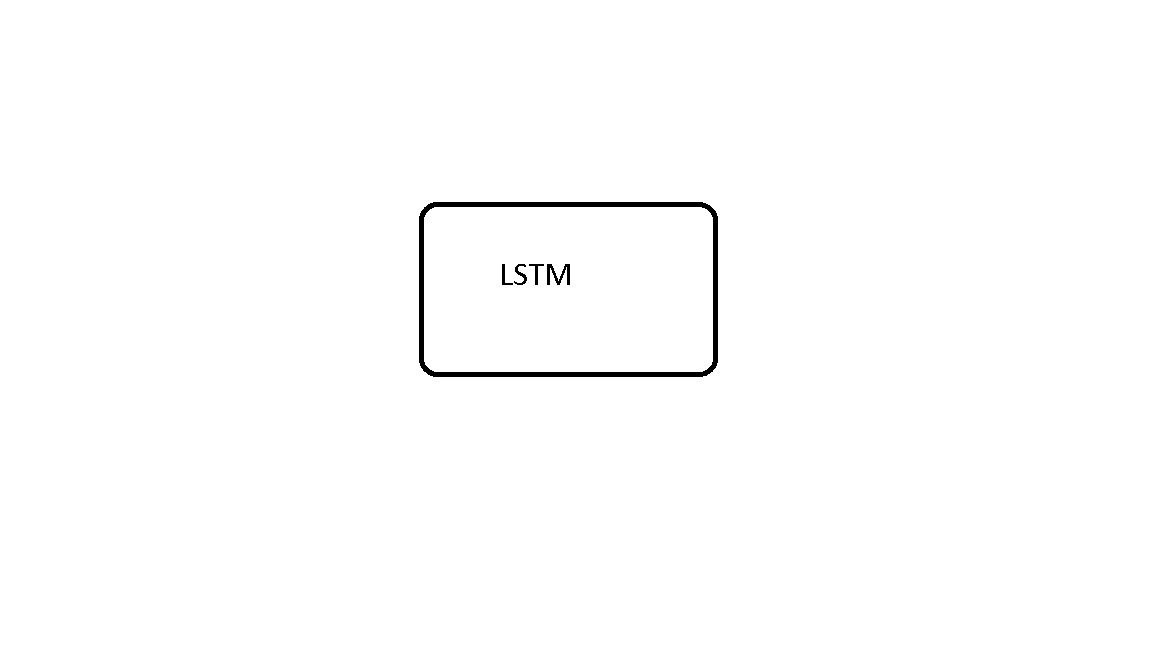
\includegraphics[width=0.25\textwidth]{imgs/LSTM-diagrama.jpg}
    \label{fig:diagrama-LSTM}
    \caption{Diagrama basico red LSTM.}
\end{figure}

Este tipo de redes son las más utilizadas actualmente para realizar reconocimiento de caracteres, pero cuentan con la desventaja de una alto costo computacional, lo que hace que se uso sea desaconsejable en sistemas embedidos.

La otra alternativa que se utiliza es la de Redes Neuronales del tipo convulucional, que mediante filtros bidimensionales y una serie de capas totalmente conectadas se predice el texto más probable.
Al no requerir almacenar información ni trabajar de forma recursiva, la implementación
de este tipo de redes pueden ser implementadas en equipos con un hardware de menor potencia,menor tamaño y por consiguiente menor costo. La mayor desventaja es que el tamaño del texto debe estar previamente definido.
\begin{figure}[h]
    \centering
    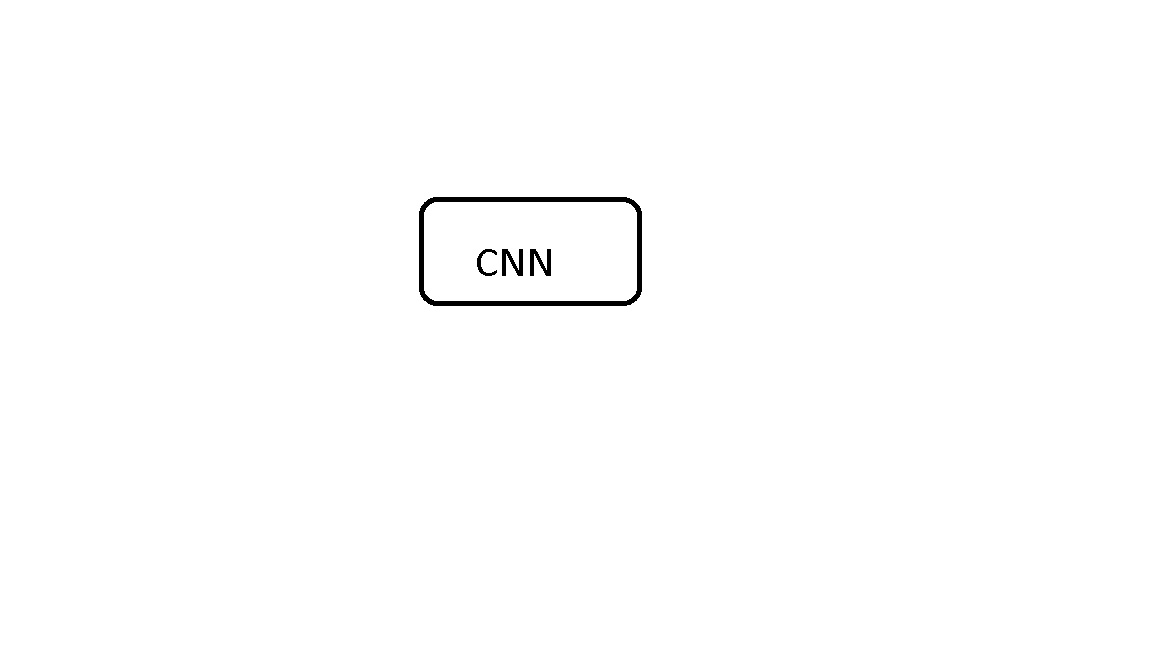
\includegraphics[width=0.25\textwidth]{imgs/CNN-diagrama.jpg}
    \label{fig:diagrama-CNN}
    \caption{Diagrama simplificado de una red con capas de convolución.}
\end{figure}

Debido a que las patentes tanto las lanzadas en 1994 y 2015 en Argentina Fig. \ref{fig:patentes-arg} puden ser consideradas de siete caracteres contando el último caracter de las de 1994 como un ``\_", es posible construir una red capaz de correr en hardware embedido, y es por ello que se opto por una red que implemente capaz de convolución sobre la opción de la LSTM.

\begin{figure}[h]
    \centering
    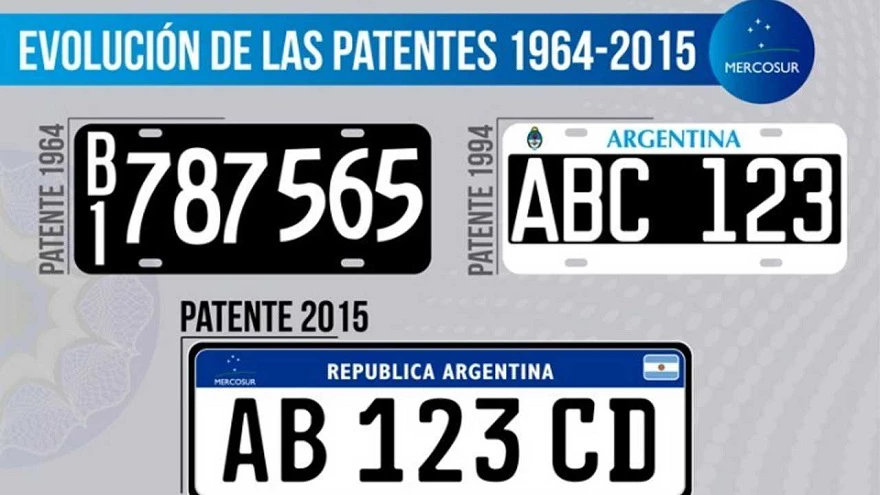
\includegraphics[width=0.5\textwidth]{imgs/patentes-arg.png}
    \caption{Evolución patentes Argentinas a lo largo de los años.}
    \label{fig:patentes-arg}
\end{figure}


\section{Qué es una red neuronal?}

Se entiende como red neuronal a un algoritmo computacional que intenta imitar el cerebro humano, en otras palabras es un algoritmo de computación compuesto por un gran número de elementos simples que se
encuentran interconectados, los cuales procesan la información por medio de estados dinámicos, respondiendo a entradas externas, que permite realizar diversas tareas.
En este caso se centrara el trabajo a la tarea de claficación de datos.
Debido a la semenjanza que existe entre los algoritmos de Deep Learning (algoritmos de aprendizaje profundo o
Machine learning [Referencia https://www.ibm.com/topics/machine-learning] compuesto por redes neuronales
de 3 o mas capas)[Referencia https://www.ibm.com/es-es/topics/deep-learning] y el cerebro humano, a la
unidad fundamental de estos sistemas se la denomina neurona.


\subsection{La neurona}

La neurona es la unidad fundamental dentro de la red, y su nombre viene debido a la similud que existe entre este elemento y una neurona humana, esta similitud se puede apreciar en Fig. \ref{fig:comparativa-neuronas}. La tarea de la neurona es procesar la información información que le entra para producir un valor de salida, a este proceso se lo conoce como sinapsis.

\begin{figure}[h]
    \centering
    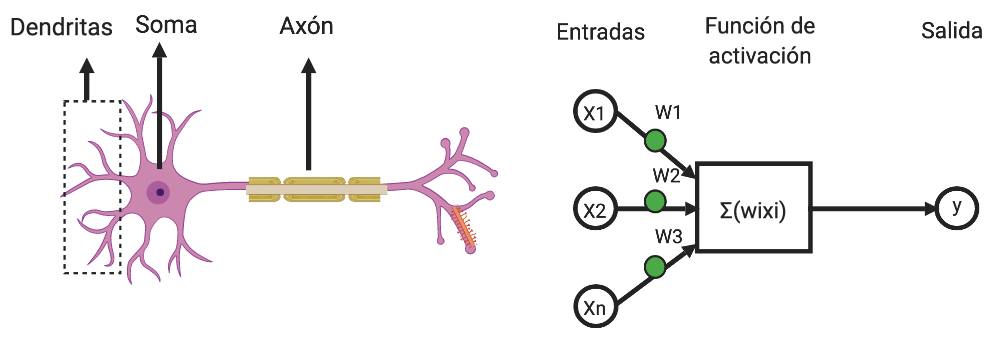
\includegraphics[width=1\textwidth]{imgs/comparacion-neurona-red.png}
    \caption{Comparacion neurona biologica con nuerona artificial.}
    \label{fig:comparativa-neuronas}
    %https://futurelab.mx/redes%20neuronales/inteligencia%20artificial/2019/06/25/intro-a-redes-neuronales-pt-1/
\end{figure}

La sinapsis entre nueronas es una suma poderada que puede ser expresada como $y =W^T X + b$ donde $y$ es el valor de salida de la nuerona,
$W$ representa los pesos de la neurona y se define como un vector columna de dimensión $N$, $b$ es un bias y $X$ es el vector columna de dimensión $N$. Si bien la neurona es muy util, sola no es de mucha utilidad, es por ello que a los arreglos en paralelo de neuronas se los denomina capa, a las capas de neuronas simples se las denomina capas totalmente conectadas.

\section{La red neuronal}

A la hora de resolver problema complejos es usual necesitar más de una capa, es por ello que es posible interconectar capas para formar una red neuronal en la Fig. \ref{fig:esquema-redes} se observa una red con más de una capa. La interconexión se realiza pasando toda los resultados de la capa anterior como entrada de la capa siguiente.

\begin{figure}[h]
    \centering
    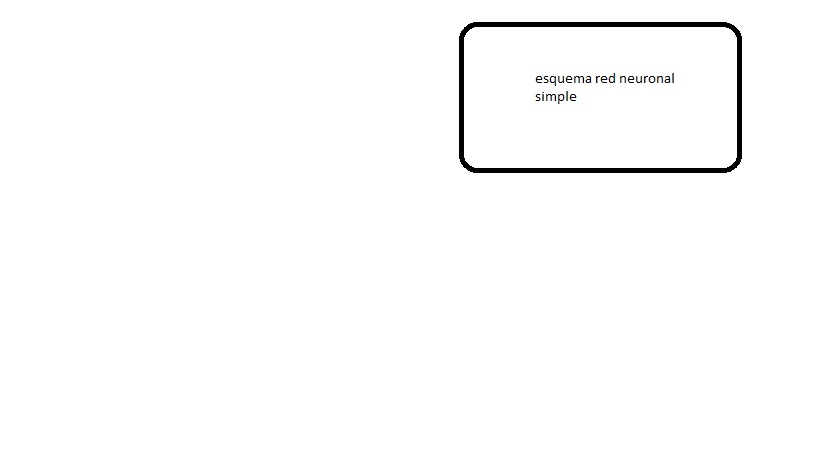
\includegraphics[width=0.5\textwidth]{imgs/Redes-esquema.jpg}
    \caption{Esquema simplificado de una red neuronal.}
    \label{fig:esquema-redes}
\end{figure}

Debido a que en esencia el proceso que realiza la neurona es una transformación lineal, al interconectar capas la resultante sigue siendo una transformación lineal.
Este problema de linealidad se soluciona aplicando una transformacion no lineal, la cual se suele llamar función de activación,
luego de que la información es procesada por la neurona, obteniendo $y= f(W^T X + b)$, las funciones de activación más conocidan se pueden observar en la
Fig. \ref{fig:funciones-activacion}.

\begin{figure}
    \centering
    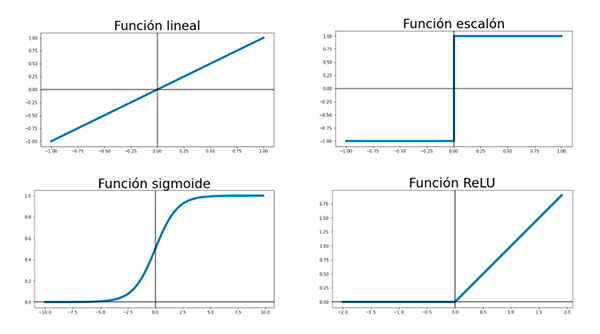
\includegraphics[width=1\textwidth]{imgs/Funciones-de-activacion.jpg}
    \caption{Funciones de activacion más comunes.}
    \label{fig:funciones-activacion}
\end{figure}

{
\huge REEVER esta parte
}

En forma resumida podemos decir que la red funciona de la siguiente manera, se realiza la multiplacion de la entrada y los pesos de la red,
luego los resultados son ingresados a la funcion de activacion para quitar las linealidades, a su vez se calcula una funcion de costo que se obtiene
con los valores obtenidos y los que se espera obtener, esta funcion es usada principalmente en el ajuste de los pesos de la red, es decir el
entrenamiento de la misma.

\section{La red neuronal de convolución}

Si bien, hasta ahora hemos visto solo las capas totalmente conectadas existen una gran cantidad de capas diferentes, para este trabajo daremos una breve introducción las redes de convolución que desde ahora llamaremos CNN.

La función principal de las capas de convolución es poder extraer información de una imagen, es por ello que nace la semenjanza entre las CNN y la corteza visual de los animales.
Este tipo de redes poseen caracteristicas que las hacen unicas, por lo que
estudiaremos las partes que la componen y en Fig. \ref{fig:esquema-CNN} se observa un esquema de la misma.
\begin{itemize}
    \item Capa convolucional: capa principal de las CNN, sus parametros son basicamente filtros entrenables de dimesiones determindas por el
          usuario,realizando una multiplicación punto a punto recorriendo toda la imagen y produciendo un mapa de activacion bidimensional, en otras palabras otra imagen, en la
          Fig. \ref{fig:esquema-capa-convolucional} se ve el funcionamiento de esta capa. Cada uno de estos filtros se activara segun la caracteristica que aprenda la red.
    \item Capa de agrupación: se coloca entre las capas de convolucion, toma los mapas de caracteristicas producidos por la capa de
          convolucion y los agrupa en una imagen. En esta capa se produce una reduccion de la dimesión, lo que reduce la complejidad para evitar el sobreajuste de los parametros.
    \item Función de activación.
    \item Capa de aplanamiento o Flatten: Antes de pasar las salidas de las capas convolucionales se produce un aplanamiento de las imagenes, esta capa transforma las imagen o matrices de dimensión $NxN$ en un vector columna $2NM$ donde $M$ es la cantidad de filtros de la capa anterior.
    \item Capa completamente conectada: Se encargan de procesar la información de los filtros para obtener la cantidad de salidas esperadas.
\end{itemize}

Si bien la descripción de las capas de convolución, agrupación y función de activación se realizaron de forma separa, se implementan juntas, ya que es común tener varias capas de convolución conectadas en serie, permitiendo extraer información más especifica de la red.

\begin{figure}
    \centering
    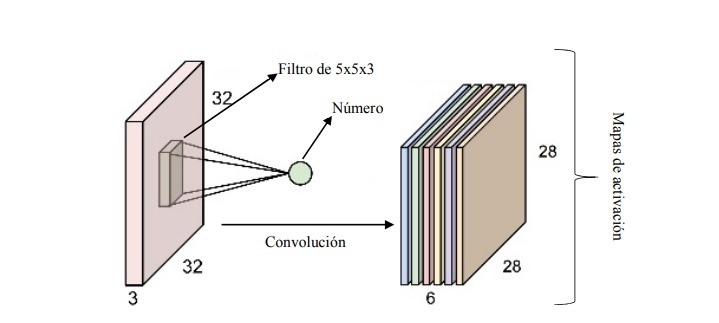
\includegraphics[width=1\textwidth]{imgs/capa-convolucional.jpeg}
    \caption{Esquema de funcionamiento de una capa convolucional.}
    \label{fig:esquema-capa-convolucional}
\end{figure}
\begin{figure}
    \centering
    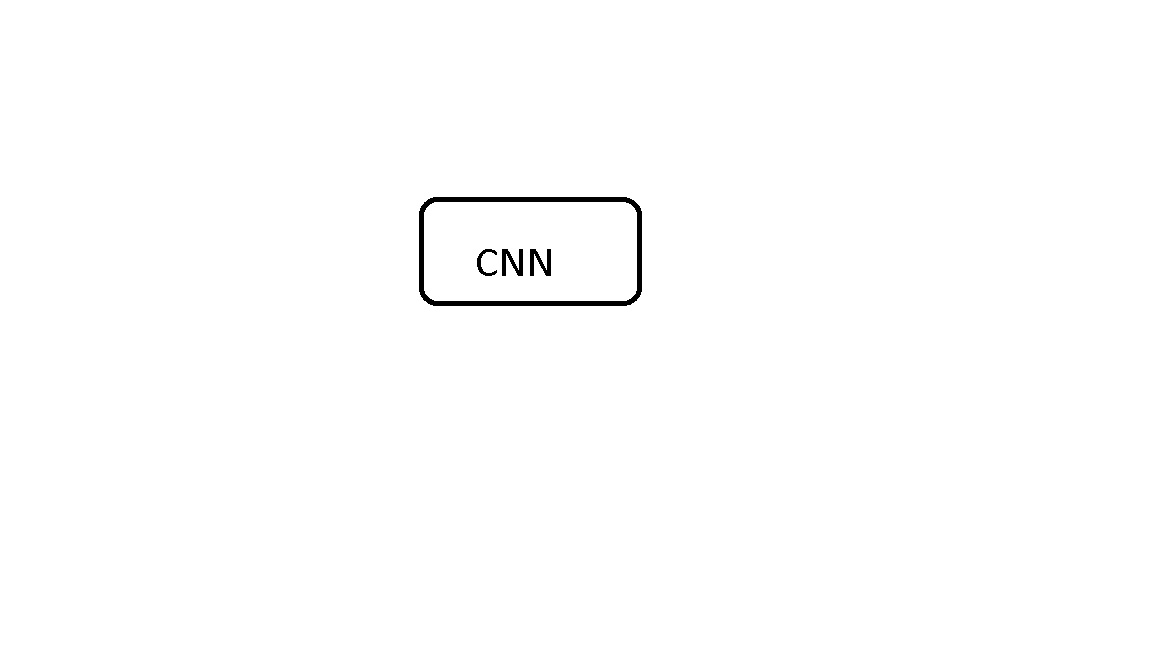
\includegraphics[width=1\textwidth]{imgs/CNN-completa.jpg}
    \caption{Esquema de un red del tipo CNN.}
    \label{fig:esquema-CNN}
\end{figure}

\subsection{Convolución en 2D}

Antes de continuar haremos una pausa para explicar el comportamiento de la convolución bidimensional, es similar al caso conocido en 1D pero
en este caso se desplaza una submatriz de un tamaño predefinido, comunmente denonimado kernel.

Se define filtro, o kernel a la respuesta de un sistema discreto, el filtro es de dimensión $2k \times 2k$ donde $k$ es un
valor establecido arbitrario (usualmente se utilizan matrices de $3 \times 3$ o $5 \times 5$) que define cuantos valores habra de la muestra.

Se define a $h[n,m]$ como un filtro de dimension $2k \times 2k$ e $I$ una imagen a escala de grises, donde cada punto de coordenadas $(i,j)$ es el
resultado de la convolucion entre $h$ e $I$ dado por
\begin{equation}
    O(i,j)= \sum_{u=-k}^{k} \sum_{v=-k}^{k} h[u,v]I[i-u,j-v]
\end{equation}

{
\huge Ver esto
}

Esta operacion consiste en filtrar una imagen de dimension $(2k+1)\times(2k+1)$ en la imagen $I$ para cada pixel centrado en dicha imagen,
calculando la operacion de convolucion.
El ajustes de los filtros necesarios para extraer caracteristicas es un proceso largo y tedioso que no siempre conduce a los
resultados que uno esperaria, por lo que es usual utilizar tecnicas machine learning para obtener los valores óptimos de los filtros.

\subsection{Capa de agrupación}

La capa de agrupación o pooling se encarga de reducir el tamaño de la imagen ejecutando una función a una submatriz de $n \times n$ de la imagen pasando de tener un elemento, las funciones de polling más utilizadas son:

\begin{itemize}
    \item MaxPooling: se queda con el valor máximo de la submatriz.
    \item AveragePooling: calcula la media de los elementos.
\end{itemize}

Otra forma de entender a la capa de pooling es un submuestro de la imagen de salida de la capa de convolución y devuelve el un valor más significativo.

En la Fig. \ref{fig:ejemplo-mp} se puede apreciar el comportamiento de una capa de maxpooling, luego de la capa de convolucion, se divide la matriz
en pequeñas matrices de $2 \times 2$ para este caso y se extrae el valor mas representativo de cada submatriz, reduciendo la matriz del ejemplo de un tamaño de
$5 \times 5$ a una de $3 \times 3$.
\begin{figure}
    \centering
    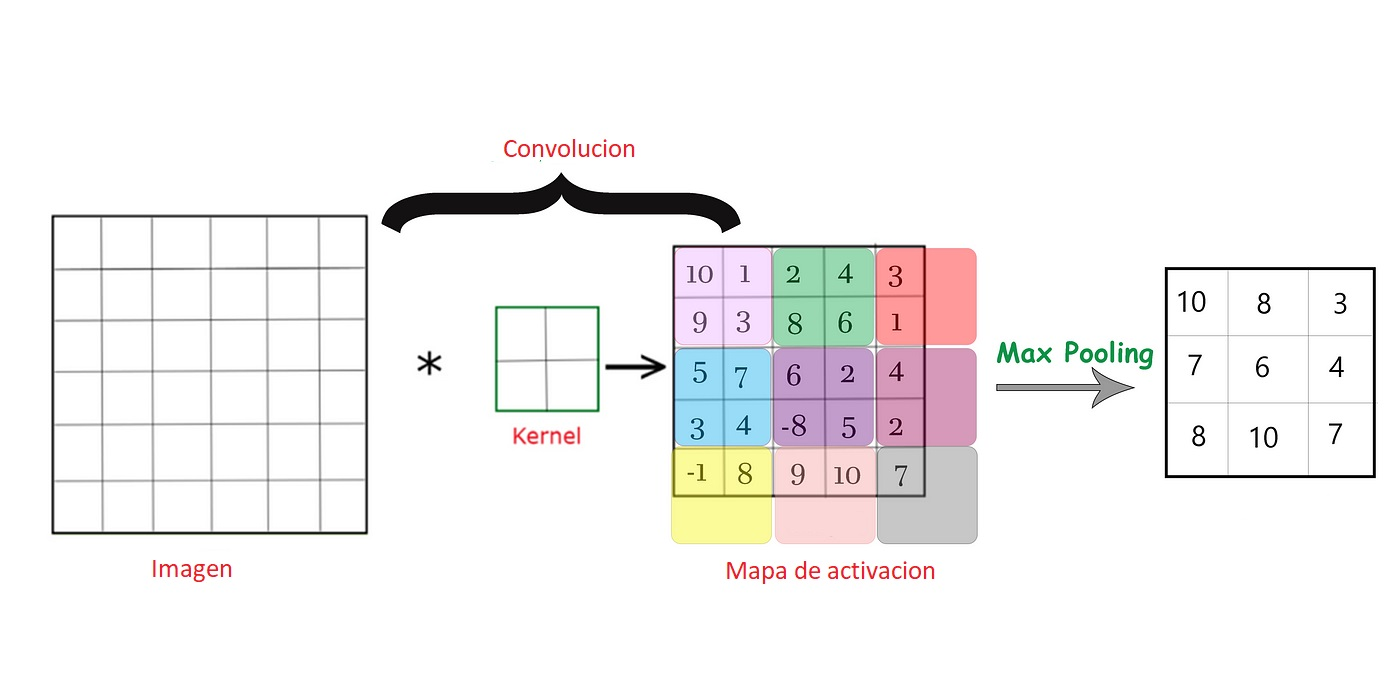
\includegraphics[width=1\textwidth]{imgs/ej-maxpooling.jpg}
    \caption{Ejemplo de funcionamiento de Maxpooling.}
    \label{fig:ejemplo-mp}
\end{figure}

\subsection{Técnica de Batch-Normalization}

La técnica de Batch-Normalization se utiliza para reducir la covarianza de los datos de entrada, esto se realiza normalizando los datos de entrada en un rango de 0 a 1 evitando trabajar con numeros grandes. Si bien este proceso se suele realizar con los datos de entrada, es útil realizarlo entre capas antes de la función de activación para trabajar siempre con datos normalizados, lo que permite que un ajuste de parámetros más simple. Finalmente antes de pasar a la capa siguiente se aplica la función de activación.

\section{CCN-OCR}

Para este trabajo se utilizó una CNN diseñada y entrenada por Ankadrew, cuya arquitectura puede verse en Fig. \ref{fig:arquitectura-cnn-ocr}. De la arquitectura de la red se destaca la capa de Global Average Pooling, la cual remplaza a la capa de aplanamiento y calcula la media por cada imagen de salida de la capa anterior, produciendo un valor por cada imagen [incluir figura de la diferencia de un flatten y un global average pooling].
\begin{figure}
    \centering
    \caption{Arquitectura de la CNN.}
    \label{fig:arquitectura-cnn-ocr}
\end{figure}

Otro elemento a destacar de la red son las 7 capas densas conectadas en pararelo, esto se debe a que como se anticipó en secciones anteriores, las patentes poseen sieste caracteres. En esencia cada capa densa es identica, solo se diferencian sus pesos los cuales son aprendidos durante el entrenamiento de la misma. Cada capa posee en total 37 caracteres de salida, esto surge de las 26 letras del abcedario, los 10 números del 0 al 9 y el simbolo de guion bajo (\_) utilizado en el caso de las patentes antiguas que solo poseen 6 caracteres.

Como aclaración para el resto del trabajo cada vez que se refiera a CNN-OCR nos estaremos refiriendo a esta red.

\section{Requerimientos necesarios de la red}

Si bien la CNN es muy útil para la tarea a resolver, posee una serie de requisitos previos en la imagen de entrada.
Según el autor la CNN necesita como entrada una red imagen de la patente en blanco y negro de dimensiones $70 \times 140$ pixeles.
Por lo que es necesario realizarle un tratamiento previo a las imagenes obtenidas antes de ingresalas por la CNN-OCR, el tratamiento necesario se puede observar en la Fig. \ref{fig:Comparativa-imagenes}. Por lo que existen 3 pasos previos luego de sacar la captura antes de ingresarla a la CNN-OCR:

\begin{enumerate}
    \item Obtener un recorte de la patente.
    \item Transformar la imagen a escala de grises.
    \item Redimensionar la imagen al tamaño requerido.
\end{enumerate}
\begin{figure}[!tbp]
    \centering
    \begin{subfigure}[b]{0.49\textwidth}
        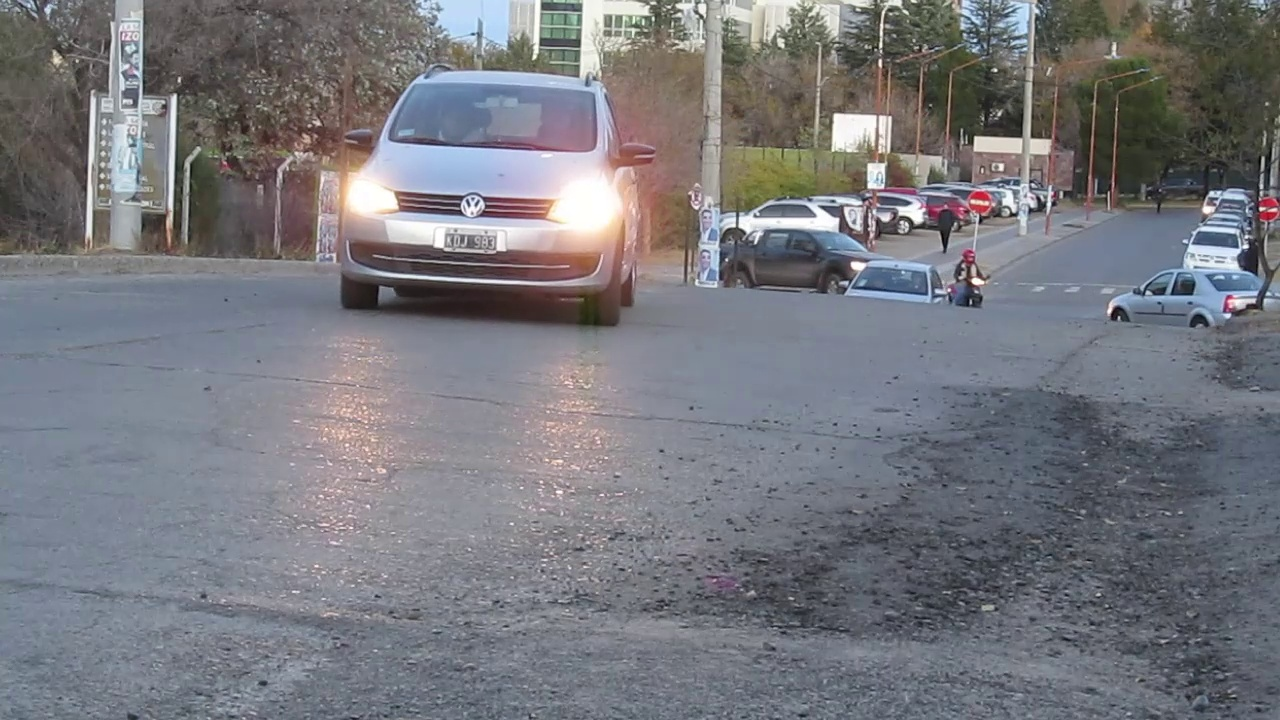
\includegraphics[width=\textwidth, height=\textwidth]{imgs/imagen-obtenida.jpg}
        \caption{Imagen obtenida por la camara.}
        \label{fig:imagen-obtenida}
    \end{subfigure}
    \hfill
    \begin{subfigure}[b]{0.49\textwidth}
        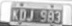
\includegraphics[width=0.7\textwidth, height=0.7\textwidth]{imgs/imagen-requerida.jpg}
        \caption{Imagen requerida por la red.}
        \label{fig:imagen-requerida}
    \end{subfigure}
    \caption{Compartiva imagenes a) Obtenida por la camara b) Requerida por la red.}
    \label{fig:Comparativa-imagenes}
\end{figure}

\subsection{Obtención del recorte de la patente}

Para lograr obtener el recorte, el autor de la CNN-OCR recomienda utilizar otra red para que detecte la ubicación de la patente, para luego ingresarla a la CNN-OCR para que obtenga los caracteres, dicha red es la Yolo (You Only Look Once) en su versión 4 desde ahora en más a esta arquitectura se le llamará YoloV4. [agregar link a github de la yolo]

El modelo de la YoloV4 es un sistema de código abierto el cual se centra en la detección de objetos, el cual utiliza una CNN con la arquitectura Darknet [incluir link a la arquitectura]. El objetivo de este algoritmo es encontrar una caja que contenga el objeto a indentificar, para este trabajo la implementación de la YoloV4 buscara la ubicación de patentes en la imagen, siendo capaz de detectar más de una patente por imagen. Para llevar a cabo la tarea de reconociento por bloques,

Este difiere con otro tipo de detectores en que no utiliza la imagen completa y se queda con las regiones en la que obtuvo mayor puntaje y las
considera como objeto detectado si no que, mediante una red neuronal tambien del tipo CNN toma la imagen completa, dibuja una serie de cuadrados
en diversas capas junto con su clasificacion, estas capas deben mesclarse para realizar la correcta deteccion, dicha implementacion se ve en la
Fig. \ref{fig:funcionamiento-yolo}, una vez que se tiene la ubicacion del objeto una CNN clasifica la imagen. Esta implementación de YoloV4.
\begin{figure}
    \centering
    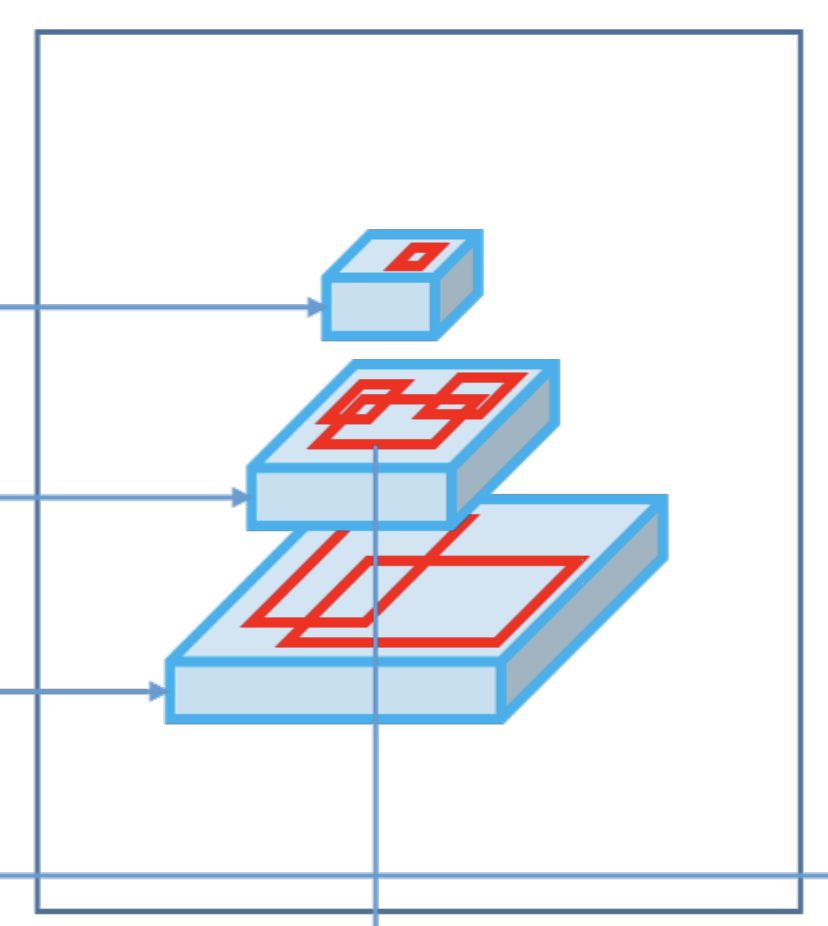
\includegraphics[width=0.5\textwidth]{imgs/funcionamiento-yolo.png}
    \caption{Funcionamiento del proceso de deteccion de la YoloV4.}
    \label{fig:funcionamiento-yolo}
    %%https://blog.roboflow.com/a-thorough-breakdown-of-yolov4/
\end{figure}

\section{Implementación del algoritmo en Python 3}

Para la implementación del algoritmo se utilizó el lenguaje Python 3, ya que este permite una rapida integración de diversas librerias necesarias para el funcionamiento del sistema completo. La implementación del algoritmo se puede observar en Fig. \ref{fig:algoritmo-ocr}, se describe de forma general.

\begin{figure}
    \centering
    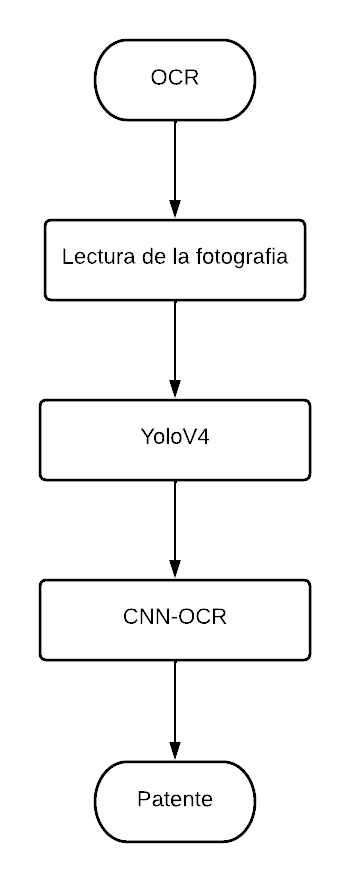
\includegraphics[width=.25\textwidth]{imgs/flujo-algoritmo-ocr.png}
    \caption{Algoritmo general de OCR.}
    \label{fig:algoritmo-ocr}
\end{figure}

La lectura u obtención de una fotografía se realizó mediante OpenCV [https://github.com/opencv/opencv] ya que permite utilizar una gran varidad de fuentes tales como cámaras y archivos. Luego se procesa la YoloV4 mediande el comando

Entonces la primer parte del algorimo se basa en la obtencion de la imagen, se espera la activacion del sensor mediante un umbral programable
por el usuario y dependiendo de la ubicacion del conjunto sensor-camara, una vez que un vehiculo se detecta, se toma una imagen que dependiendo
del equipo que se este utilizando ya sea sensor SL o sensor SL mini, la existencia de estos 2 dispositivos se vera mejor en la siguiente
seccion,se realizan 2 posibles acciones, en el caso del sensor SL, por su capacidades de hardware pueden correr dentro de el ambas redes, por lo
que el procesamiento de la imagen se realiza dentro de la propia placa, y se envia a un servidor sola la informacion relevante, como lo es la patente y
la fecha y hora de ingreso o egreso dependiendo donde se encuentre el sensor. En el caso del sensor SL mini cuyas prestaciones de computo son
inferiores este solo se encarga de tomar la foto y enviarla al servidor para que este procese la imagen y devuelva al sensor la habilitacion para el
ingreso o egreso.

En ambos casos la secuencia del algoritmo es la siguiente:
\begin{itemize}
    \item cada un tiempo periodico se chequea si ingreso una nueva imagen para procesarla, esto se realiza mirando el contenido de una carpeta especifica.
    \item Cuando se encuentra una nueva imagen, se ingresa la imagen a la YoloV4, para que detecte la ubicacion de la patente, aqui ocurren 2 posibles acciones, si
          se detecto patente se obtiene las coordenadas para realizar el recorte y en el caso de no detectar patente se envia un codigo de error al servidor y se descarta la imagen.
    \item se realiza el recorte de la imagen.
    \item Se envia la imagen de la patente recortada para la que la CNN realice la deteccion de caracteres.
    \item obtenida la patente se envia al servidor para los chequeos de validacion, y registro de horario.
    \item se recibe del servidor la validacion, y se admite la circulacion del vehiculo.
\end{itemize}




